\documentclass[11pt, addpoints, answers]{exam}

\usepackage{amsmath, amssymb}
\usepackage{xcolor}
\usepackage{drawstack}
\usepackage{physics}

\newcommand{\red}[1]{\textcolor{red}{#1}}

% For inserting code snippets.
\usepackage{listings}
\lstset{
    columns = fixed,
    basewidth = {0.5em},
    breaklines = true,
    backgroundcolor = \color{white},
    keywordstyle = \color[RGB]{40, 40, 255},
    numberstyle = \footnotesize\color{darkgray},
    commentstyle = \ttfamily\color{violet},
    basicstyle = \ttfamily,
    stringstyle = \ttfamily\color[RGB]{128, 0, 0},
    showstringspaces = false,
    language = {[11]C++},
    escapechar = \@
}
\lstnewenvironment{cpp}[1][]{\lstset{language = {[11]C++}, #1}}{}

\usepackage{tikz}
\usepackage{algorithmicx}

% headers, footers, titles
\newcommand{\CourseName}{CS101 Algorithms and Data Structures}
\newcommand{\HomeworkNO}{Homework 9}
\newcommand{\DueDate}{Due date: December 18, 2023, at 23:59}

\pagestyle{headandfoot}
\runningheadrule
\runningheader{\CourseName}{\HomeworkNO}{\DueDate}
\runningfooter{}{\thepage}{}

\title{
    \CourseName\\
    Fall 2023\\
    \HomeworkNO
}
\author{}
\date{\DueDate}

% formats of questions, choices, points, etc.
\qformat{\textbf\thequestion. (\totalpoints\ points) \thequestiontitle\hfill}
\pointname{'}
\CorrectChoiceEmphasis{\color{blue}}
\SolutionEmphasis{\color{blue}}

% We frequently use this font.
\newcommand{\ttt}{\texttt}
\newcommand{\bluett}[1]{\textcolor{blue}{\ttt{#1}}}

\begin{document}

    \maketitle

    \begin{enumerate}
        \item Please write your solutions in English.
        \item Submit your solutions to gradescope.com.
        \item Set your FULL name to your Chinese name and your STUDENT ID correctly in Account Settings.
        \item If you want to submit a handwritten version, scan it clearly. \ttt{CamScanner} is recommended.
        \item When submitting, match your solutions to the problems correctly.
        \item No late submission will be accepted.
        \item Violations to any of the above may result in zero points.
    \end{enumerate}

    \begin{questions}

        \newpage

        \titledquestion{Multiple Choices}

Each question has \textbf{one or more} correct answer(s). Select all the correct answer(s). For each question, you will get 0 points if you select one or more wrong answers, but you will get 1 point if you select a non-empty subset of the correct answers.

Write your answers in the following table.

%%%%%%%%%%%%%%%%%%%%%%%%%%%%%%%%%%%%%%%%%%%%%%%%%%%%%%%%%%%%%%%%%%%%%%%%%%%
% Note: The `LaTeX' way to answer a multiple-choices question is to replace `\choice'
% with `\CorrectChoice', as what you did in the first question. However, there are still
% many students who would like to handwrite their homework. To make TA's work easier,
% you have to fill your selected choices in the table below, no matter whether you use 
% LaTeX or not.
%%%%%%%%%%%%%%%%%%%%%%%%%%%%%%%%%%%%%%%%%%%%%%%%%%%%%%%%%%%%%%%%%%%%%%%%%%%

\begin{table}[htbp]
    \centering
    \begin{tabular}{|p{2cm}|p{2cm}|p{2cm}|p{2cm}|}
        \hline
        (a) & (b) & (c) & (d) \\
        \hline
        %%%%%%%%%%%%%%%%%%%%%%%%%%%%%%%%%%%%%%%%%%%%%%%%%%%%%%%%%%
        % YOUR ANSWER HERE.
        AD  & BCD & AB  & D   \\
        %%%%%%%%%%%%%%%%%%%%%%%%%%%%%%%%%%%%%%%%%%%%%%%%%%%%%%%%%%
        \hline
    \end{tabular}
\end{table}

\begin{parts}
    \part[2] Which of the following operations on a \textbf{Linked List} take constant time?

    \begin{choices}
        \CorrectChoice Given a pointer $h$ which points to the head node of a linked list, we want to erase the head node.
        \choice Given a pointer $h$ which points to the head node of a linked list, we want to gain access to the last element of the linked list.
        \choice Given a pointer $p$ which points to a node in a linked list, we want to gain access the previous node of $p$.
        \CorrectChoice Given a pointer $p$ which points to a node in a linked list, we want to insert an element after $p$.
    \end{choices}

    \part[2] Which of the following statements about arrays and linked-lists are true?

    \begin{choices}
        \choice Inserting an element into the middle of an array takes constant time.
        \CorrectChoice A doubly linked list consumes more memory than a (singly) linked list of the same length.
        \CorrectChoice Given a pointer to some node in a doubly linked list, we are able to gain access to every node of it.
        \CorrectChoice Given a pointer to any node in a linked list, we are able to gain access to the last node.
    \end{choices}

    \part[2] Please evaluate the following reverse-Polish expressions. Which of them are legal reverse-Polish expressions and gives a result greater than 0?

    \begin{choices}
        \CorrectChoice \ttt{2 3 2 * + 1 /}
        \CorrectChoice \ttt{1 2 4 - - 3 *}
        \choice \ttt{1 * 2 - 1 + 5}
        \choice \ttt{2 4 3 1 + * -}
    \end{choices}

    \part[2] Assume we implement a queue with a circular array indexed from $0$ to $n-1$. Now the \ttt{front} pointer is at index $a$, and the \ttt{back} pointer is at index $b$. Which of the following best describes the number of the elements in the queue?

    \begin{choices}
        \choice $b-a+1$
        \choice $|b-a+1|$
        \choice $b-a+1+n$
        \CorrectChoice $(b-a+1+n) \mod n$
    \end{choices}


\end{parts}

        \newpage

        \titledquestion{Topological Sort}

Given the following DAG, run topological sort with a queue. Write down the vertex you select and update the in-degree \texttt{ind[i]} of all vertices in each iteration.

\textit{Note: When pushing several vertices into the queue at the same time, push them alphabetically. You are NOT required to show your queue at each step.}

\vspace{1cm}

\begin{figure}[htbp]
    \centering
    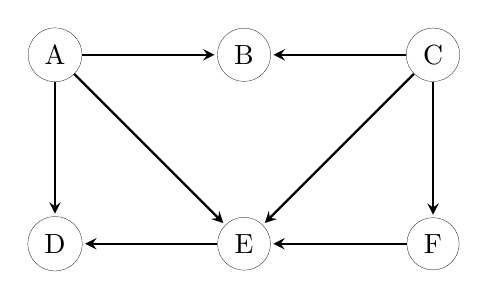
\begin{tikzpicture}[
        > = stealth, % arrow head style
        shorten > = 1pt, % don't touch arrow head to node
        node distance = 1cm, % distance between nodes
        thick, % line style
        scale = 0.8,
    ]
        % Draw the nodes
        \foreach \pos/\i in {
            (-3,3)/A,
            (0,3)/B,
            (3,3)/C,
            (-3,0)/D,
            (0,0)/E,
            (3,0)/F} {
            \node[circle, draw, line width=0.1pt] (\i) at \pos {\i};
        }

        % Draw the edges
        \foreach \b/\e in {
            A/B,
            A/D,
            A/E,
            C/B,
            C/E,
            C/F,
            F/E,
            E/D} {
            \draw[->] (\b) to (\e);
        }
    \end{tikzpicture}\label{fig:Topological_Sort}
\end{figure}
\vspace{0.5cm}

\begin{table}[htbp]
    \begin{center}
        \begin{tabular}{|l|c|l|l|l|l|l|l|}
            \hline
            & vertex & \texttt{ind[A]}    & \texttt{ind[B]}    & \texttt{ind[C]}    & \texttt{ind[D]}    & \texttt{ind[E]} & \texttt{ind[F]}\\ \hline
            initial     &  /      & \textcolor{blue}{0} & \textcolor{blue}{2} & \textcolor{blue}{0} & \textcolor{blue}{2} & \textcolor{blue}{3} & \textcolor{blue}{1}   \\ \hline
            iteration 1 &   A     & \textcolor{blue}{} & \textcolor{blue}{1} & \textcolor{blue}{0} & \textcolor{blue}{1} & \textcolor{blue}{2} & \textcolor{blue}{1}   \\ \hline
            iteration 2 &   C     & \textcolor{blue}{} & \textcolor{blue}{0} & \textcolor{blue}{} & \textcolor{blue}{1} & \textcolor{blue}{1} & \textcolor{blue}{0}   \\ \hline
            iteration 3 &   B     & \textcolor{blue}{} & \textcolor{blue}{} & \textcolor{blue}{} & \textcolor{blue}{1} & \textcolor{blue}{1} & \textcolor{blue}{0}   \\ \hline
            iteration 4 &   F     & \textcolor{blue}{} & \textcolor{blue}{} & \textcolor{blue}{} & \textcolor{blue}{1} & \textcolor{blue}{0} & \textcolor{blue}{}   \\ \hline
            iteration 5 &   E     & \textcolor{blue}{} & \textcolor{blue}{} & \textcolor{blue}{} & \textcolor{blue}{0} & \textcolor{blue}{} & \textcolor{blue}{}   \\ \hline
            iteration 6 &   D     & \textcolor{blue}{} & \textcolor{blue}{} & \textcolor{blue}{} & \textcolor{blue}{} & \textcolor{blue}{} & \textcolor{blue}{}   \\ \hline
        \end{tabular}
    \end{center}\label{tab:Topological_Sort_Answer}
\end{table}
\vspace{0.5cm}



\begin{parts}
    \part[3] Fill in the table above.
    \part[2] What is the topological order that you obtain?
    \begin{solution}
        A, C, B, F, E, D
    \end{solution}
    \part[3] How many different topological orders starting with A does this graph have?
    Write them down.
    \begin{solution}
        \\
        2 \\
        A, C, B, F, E, D\\
        A, C, F, B, E, D
    \end{solution}
\end{parts}

        \newpage

        \titledquestion{Array Section: Maximal Power}

Given a sequence of positive integers $A=\langle a_1,\cdots,a_n\rangle$, we want to divide it into several consecutive sections so that the sum of power of these sections
is maximized.

The power of section $\langle a_i,\cdots,a_j\rangle$ is defined as $aX_{i,j}^2+bX_{i,j}+c$, where
\begin{itemize}
    \item $a,b,c$ are given constants.
    \item $X_{i,j}=\sum\limits_{k=i}^j a_k$ is the sum of values in the section.
\end{itemize}

Please design a \textbf{dynamic programming} algorithm that returns the maximal sum of power of the sections that you divided.

For example, if \(a=-1,b=10,c=-20\) and \(A=\langle 2,2,3,4\rangle\), the maximal sum of power is \(9\), and the way to divide the sequence is: \(\langle 2,2\rangle,\langle 3\rangle,\langle 4\rangle\).

\begin{parts}
    \part[3] Define the subproblems for $i\in[0,n]$: $OPT(i)=$ the maximal sum of power of if you only consider dividing the first $i$ elements. Give your Bellman equation to solve the subproblems.
    \begin{solution}
        $$
            OPT(i) = \begin{cases}
                0                                                                 & \text{if } i = 0 \\
                \max_{1 \leq j \leq i} \{ OPT(j-1) + aX_{j,i}^2 + bX_{j,i} + c \} & \text{if } i > 0 \\
            \end{cases}
        $$
    \end{solution}

    \part[1] What is the answer to this question in terms of $OPT$?
    \begin{solution}
        The answer to the problem is $OPT(n)$.
    \end{solution}

    \part[3] What is the runtime complexity of your algorithm? (answer in $\Theta(\cdot)$)
    
    \textbf{Hint:} How will you compute $X_{j,i}$ in $\Theta(1)$ time? Please give your analysis of the preprocessing and computing complexity.
    \begin{solution}
        To calculate the runtime complexity, we consider the number of subproblems and the time it takes to solve each subproblem. We have $n$ subproblems corresponding to $OPT(1), OPT(2), \ldots, OPT(n)$. For each subproblem $OPT(i)$, we must compute the maximum over $i$ possible sections. The complexity of computing each section's power is $O(1)$ after preprocessing, so the complexity for each $OPT(i)$ is $O(i)$.
        
        The total complexity is the sum of the complexities for all subproblems:
        
        $$
        \sum_{i=1}^{n} O(i) = O\left(\frac{n(n+1)}{2}\right) = O(n^2)
        $$
        
        Thus, the runtime complexity of the algorithm is $\Theta(n^2)$.
                
        \pagebreak
        
        \textbf{Preprocessing and Computing Complexity:}

        To compute $X_{j,i}$ in $\Theta(1)$ time, we can preprocess the input sequence to create a prefix sum array $P$, where $P[i] = \sum_{k=1}^{i} a_k$. The preprocessing step takes $\Theta(n)$ time.

        Once we have the prefix sum array, we can compute $X_{j,i}$ using $P[i] - P[j-1]$ in constant time.

        The preprocessing complexity is $\Theta(n)$, and the overall complexity remains $\Theta(n^2)$ since this does not dominate the $\Theta(n^2)$ complexity of solving the subproblems.
    \end{solution}
\end{parts}





        \newpage

        \titledquestion{Minimum Cost Refueling}

You are planning to from city A to city B on a highway.
The distance between A and B is $d$ kilometers.
The vehicle departs with $f_0$ units of fuel.
Each unit of fuel makes the vehicle travel one kilometer.

There are $n$ gas stations along the way.
The $i$-th station is situated $p_i$ kilometers away from city A.
Note that $0<p_1<p_2<\cdots<p_n<d$.

If the vehicle chooses to refuel at the $i$-th station, $f_i>0$ units would be added to the fuel tank whose capacity is unlimited, which costs you \$$c_i$.
    You have a budget $B$, which means that the sum of costs on refueling is at most \$$B$.

    Please design a \textbf{dynamic programming} algorithm that returns \textbf{the minimum cost of refueling} to make sure the vehicle reaches the destination if the vehicle can reach the target, or returns $\varnothing$ if your budget is not enough or the fuel is not enough to support you to reach city B.

\begin{parts}
    \part[3] Define the subproblems for $i\in[0,n],j\in[0,B]$: $OPT(i, j)=$ the maximum distance you can drive if you spend \textbf{at most} \$$j$ among the first $i$ stations. Give your Bellman equation to solve the subproblems.
        \begin{solution}
            $$
                OPT(i, j) = \maxi{OPT(i-1, j)}{p_{i} + OPT(i-1, j-c_{i}),\;\case{j \geq c_{i} \text{ and } p_{i} \leq OPT(i-1, j-c_{i}) + f_{i}}}
            $$

        \end{solution}

        \part[2] What is the answer to this question in terms of $OPT$?
        \begin{solution}
            To find the minimum cost of refueling to ensure the vehicle reaches the destination, we look for the smallest $j$ such that $OPT(n, j) \geq d$. If no such $j$ exists, we return $\varnothing$.
        \end{solution}
        \part[1] What is the runtime complexity of your algorithm? (answer in $\Theta(\cdot)$)
    \begin{solution}
        The algorithm iterates over each gas station and each possible budget amount, leading to a complexity of $\Theta(nB)$, since for each $(i, j)$ pair, we compute $OPT(i, j)$ in constant time.
    \end{solution}
\end{parts}




        \newpage

        \ % The empty page

        \newpage

    \end{questions}

\end{document}